
\section{G\'{e}n\'{e}ralit\'{e}s sur le test automatique}

Pour r\'{e}pondre \`{a} la question \textquote{Qu'est-ce qu'un test automatique?}, je dirais que c'est un code v\'{e}rifiant le bon fonctionnement autre d'un code. Il existe de nombreux niveaux de test : unitaire, fonctionnel, int\'{e}gration, performance, \ldots. Les tests sont tr\`{e}s importants dans un projet logiciel, ils permettent de de s'assurer de la conformit\'{e} du logiciel par rapport aux sp\'{e}cifications (autrement dit, le besoin client). La mise en place de ces tests automatiques est facilit\'{e}e par un Framework, il en existe de nombreux mais de mani\`{e}re g\'{e}n\'{e}rale un Framework est un ensemble de librairies et de normes ( de mod\'{e}lisation, d'architecture, ...)\footnote{Source : \url{https://boulaich.wordpress.com/2009/07/08/framework-generalite/}}. \\
\subsection{Description des diff\'{e}rents types de test}

%vas voir ici!!! http://jmdoudoux.developpez.com/cours/developpons/java/chap-frameworks-test.php


\subsubsection{Le test unitaire}
Un test unitaire v\'{e}rifie le bon fonctionnement d'une petite portion de code. En r\`{e}gle g\'{e}n\'{e}rale il s'agit de tester que la valeur retourn\'{e}e par une m\'{e}thode est la bonne, ces tests sont donc impl\'{e}ment\'{e}s par les d\'{e}veloppeurs. Mais il s'agit aussi de valider le fonctionnement de la m\'{e}thode aux limites et de v\'{e}rifier la coh\'{e}rence de ses r\'{e}sultats. Ces tests sont cens\'{e}s \^{e}tre les plus nombreux possible pour couvrir le maximum de cas possibles, on appelle cela le test coverage (ou couverture de test).

\subsubsection{Le test fonctionnel}
Le test fonctionnel est ax\'{e} sur l'interaction des diff\'{e}rentes m\'{e}thodes, il est ax\'{e} sur les fonctionnalit\'{e}s du logiciel. Ces tests permettent de v\'{e}rifier le bon fonctionnement des sp\'{e}cifications du produit et de valider que les fonctionnalit\'{e}s correspondent aux sp\'{e}cifications. Ceux-ci sont assur\'{e}s par les testeurs automatiques (ST).

\subsubsection{Le test d'int\'{e}gration}
Le test d'int\'{e}gration est au test fonctionnel ce que le test fonctionnel est au test unitaire, avec plusieurs niveaux de granularit\'{e}s (plus ou moins grand nombre de m\'{e}thodes concern\'{e}es). Le test d'int\'{e}gration s'assure du bon fonctionnement du logiciel en interaction avec d'autres logiciels.

\subsubsection{Le test de performance}
Le test de performance s'assure qu'une action est effectu\'{e}e dans le temps imparti. Les actions test\'{e}es sont aux minimum celles qui composent les workflows nominaux, tant s\'{e}par\'{e}ment que simultan\'{e}ment (multi utilisateurs).

\subsubsection{Le test de stabilit\'{e}}
Le test de stabilit\'{e} permet de tester qu'un comportement est syst\'{e}matique, autrement dit qu'une m\^{e}me action implique toujours le m\^{e}me r\'{e}sultat.\\
Les tests se stabilit\'{e}s permet de s'assurer que la r\'{e}ponse est bien l\`{a} dans le temps imparti et qu'il n'y a pas d'erreurs, ceci en faisant subir une mont\'{e}e en charge des requ\^{e}tes du logiciel sur une dur\'{e}e pouvant aller de 24 \`{a} 72 heures.

\subsubsection{Le test de scalabilit\'{e}}
Le test de scalabilit\'{e} permet de s'assurer que le logiciel peut \'{e}voluer de mani\`{e}re \`{a} pouvoir offrir les m\^{e}mes performances dans un contexte d'utilisation qui a \'{e}volu\'{e}. Par exemple, dans le cas o\`{u} la charge d'utilisation double, est-il possible de modifier l'environnement client afin que les utilisateurs profitent des m\^{e}mes performances?


\subsubsection{Le test de validation de plateforme}
Ce type de test est consacr\'{e} aux logiciels destin\'{e}s \`{a} \^{e}tre utilis\'{e}s sur plusieurs plateformes. Dans syst\`{e}me d'exploitation \`{a} un autre, les comportements sont-ils les m\^{e}mes? Les fonctionnalit\'{e}s sont-elles identiques?

\section{Le test dans l'\'{e}quipe d'automatisation des tests}
Lorsque je suis arriv\'{e} dans cette \'{e}quipe, j'ai d\'{e}couvert des logiciels que je ne connaissais pas : Perforce, ASTEC, Jenkins, et d'autres. J'ai mis un peu de temps \`{a} me les approprier et \`{a} bien comprendre \`{a} quoi ils servaient exactement. La complexit\'{e} de leur environnement d'utilisation ne m'a pas facilit\'{e} la t\^{a}che. 

Pour r\'{e}sumer ce que j'ai appris sur les g\'{e}n\'{e}ralit\'{e}s de cette \'{e}quipe c'est qu'elle utilise plusieurs outils pour g\'{e}rer le code des diff\'{e}rents logiciels, poss\'{e}dant chacun plusieurs versions. Pour chacune de ces versions une suite de tests est ex\'{e}cut\'{e}e quotidiennement o\`{u} leurs codes sont h\'{e}berg\'{e}s sur le gestionnaire de code source Perforce\index{Perforce}. 

Apr\`{e}s chaque livraison de code effectu\'{e}e, le logiciel est compil\'{e} par Jenkins, son utilisation \'{e}tant principalement de v\'{e}rifier l'\'{e}tat de la compilation apr\`{e}s chaque livraison. Et, de plus, le logiciel est compil\'{e} quotidiennement par ASTEC dont les r\'{e}sultats sont automatiquement envoy\'{e}s aux personnes concern\'{e}es (cf. annexe \ref{pdf:automationResults} page \pageref{pdf:automationResults} qui pr\'{e}sente l'un des r\'{e}sultats de ces mails). L'utilisation de ASTEC dans l'\'{e}quipe est beaucoup plus large que cela mais je n'ai pas eu l'occasion de l'\'{e}tudier plus en d\'{e}tail.\\



Le testeur automatique est focalis\'{e} sur les fonctionnalit\'{e}s du logiciel. Lorsque les sp\'{e}cifications d'une nouvelle fonctionnalit\'{e} voient le jour, un plan de test est r\'{e}dig\'{e} et est envoy\'{e} \`{a} l'\'{e}quipe du test automatique. Du test plan est extrait tous les tests pouvant \^{e}tre automatis\'{e}s et ceux-ci sont impl\'{e}ment\'{e}s.\\
Je n'ai pas beaucoup particip\'{e} \`{a} cet aspect de l'\'{e}quipe, ma principale mission relevait de l'initiative \textquote{1 bug - 1 test}. Mon travail n'\'{e}tait pas de tester une nouvelle fonctionnalit\'{e} mais plut\^{o}t, une fonctionnalit\'{e} d\'{e}j\`{a} existante sur laquelle une anomalie \`{a} \'{e}t\'{e} trouv\'{e}e, soit par un client (\`{a} \'{e}viter) soit par un individu interne \`{a} SAP.\\

Le cycle de d\'{e}veloppement de l'automatisation de tests dans lequel j'ai \'{e}volu\'{e} est r\'{e}sum\'{e} (et simplifi\'{e}) figure \ref{figure:testProcess} page \pageref{figure:testProcess}. Ce cycle est celui de l'automatisation d'un test dans le cas d'une anomalie trouv\'{e}e sur une fonctionnalit\'{e} existante et pas sur une nouvelle fonctionnali\'{e}. Mon int\'{e}gration dans ce processus de d\'{e}veloppement m'a appris beaucoup, non seulement quant \`{a} la gestion d'une anomalie logicielle, mais surtout quant \`{a} la valeur est \`{a} l'utilisation du test qui peut-\^{e}tre impl\'{e}menter soit en r\'{e}ponse \`{a} une anomalie soit dans le processus initial de d\'{e}veloppement pour garantir qu'une fonctionnalit\'{e} se comporte telle qu'elle est d\'{e}crite dans les sp\'{e}cifications.\\
\begin{figure}[!ht]
  \centering
      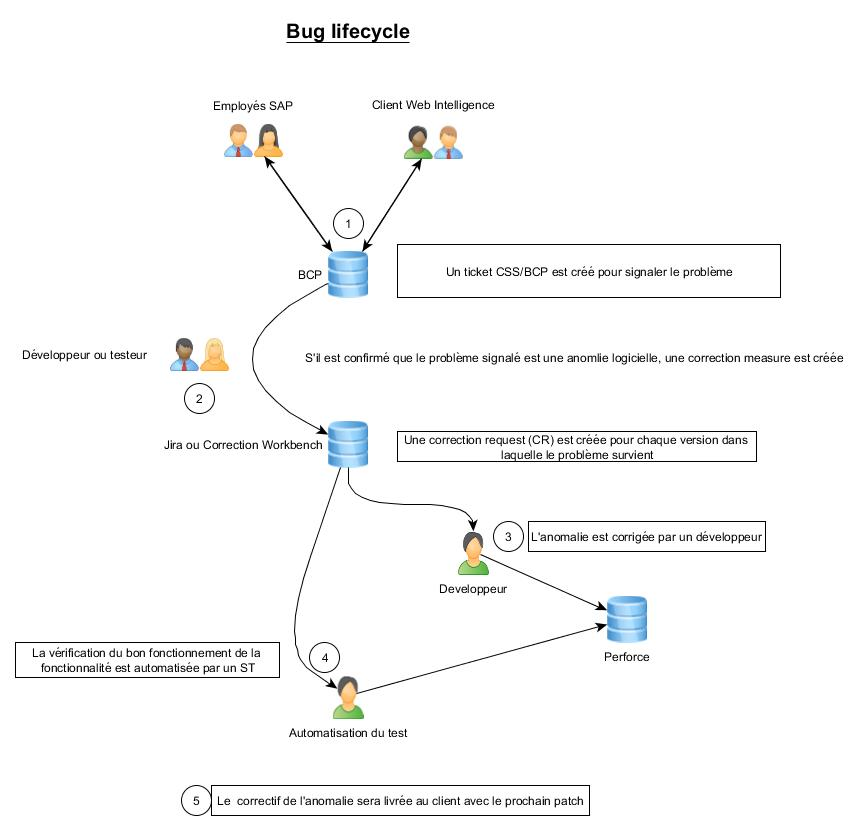
\includegraphics[width=\textwidth]{images/testProcessAtSAP.jpg}
  \caption{Le process de test}
	\label{figure:testProcess}
\end{figure}
 


\section{Pr\'{e}sentation du produit test\'{e} : Web Intelligence}
Web Intelligence est un logiciel de BI\index{Business Intelligence} permettant d'acc\'{e}der \`{a} des donn\'{e}es stock\'{e}es dans une base de donn\'{e}es. Cet acc\`{e}s aux donn\'{e}es ne se fait pas directement, tout l'int\'{e}r\^{e}t de Web Intelligence repose sur l'utilisation d'une couche s\'{e}mantique, \textquote{l'univers}.\\
Il existe trois interfaces graphiques permettant d'acc\'{e}der \`{a} ces donn\'{e}es, un client lourd et deux clients l\'{e}gers : l'applet et le client dhtml.

\section{La premi\`{e}re semaine dans l'\'{e}quipe d'automatisation des tests}






\`{A} mon arriv\'{e}e dans l'\'{e}quipe et avant de commencer \`{a} impl\'{e}menter des tests automatiques, j'ai \'{e}t\'{e} accueilli par mes coll\`{e}gues et on m'a fourni le mat\'{e}riel n\'{e}cessaire au bon d\'{e}roulement de mon travail.\\
Mes 1\up{er} jours \`{a} SAP se sont d\'{e}roul\'{e}s de la mani\`{e}re suivante :\\
\begin{itemize}
\item Pr\'{e}sentation \`{a} l'\'{e}quipe et visite des locaux
\item R\'{e}union avec mon tuteur et mon manager pour une description de la mission
\item R\'{e}cup\'{e}ration des diff\'{e}rents droits d'acc\`{e}s aux serveurs
\item Familiarisation avec les outils internes (tickets HR, CSS, IT, ...)
\item Installation des logiciels n\'{e}cessaires au d\'{e}veloppement (IDE, SCM\index{Source Code Management}, \'{e}diteur de texte, \ldots)
\item Mise en place du framework de test (cr\'{e}ation du workspace perforce)
\end{itemize}
Au terme de la 1\up{\`{e}re} semaine, j'ai pu commencer \`{a} \'{e}tudier le framework de test en me basant sur les tests d\'{e}j\`{a} existants.\\
C'est au cours de la deuxi\`{e}me semaine que j'ai pu impl\'{e}menter mes 1\up{er} tests.
